\documentclass{article}
\newcommand\tab[1][1cm]{\hspace*{#1}}
\usepackage{amssymb,amsmath,graphicx,float}
\begin{document}


  \begin{figure}
  \centering
  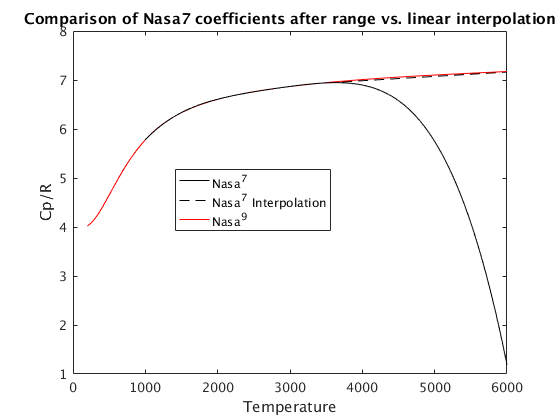
\includegraphics[width=\textwidth]{CpT.png}
  \label{fig:cpT}
  \caption{HCO comparison of Nasa 7 vs Nasa 9 data, along with linearly interpolated data for data outside of Nasa 7's range for $\frac{C_p}{T}$ data}
\end{figure}


\begin{figure}
  \centering
  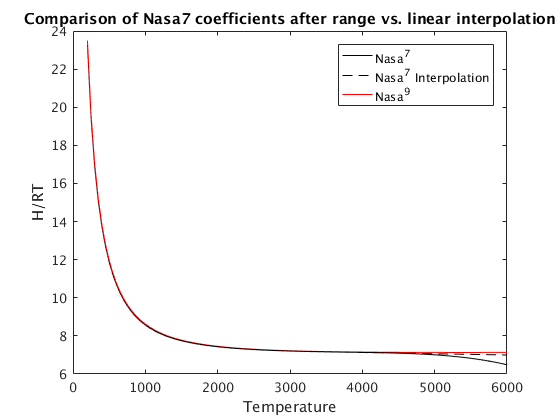
\includegraphics[width=\textwidth]{HT.png}
  \label{fig:HT}
  \caption{HCO comparison of Nasa 7 vs Nasa 9 data, along with linearly interpolated data for data outside of Nasa 7's range for $\frac{H}{RT}$ data}
\end{figure}


\begin{figure}
  \centering
  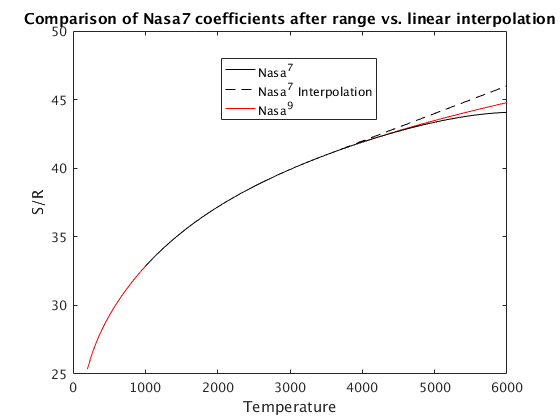
\includegraphics[width=\textwidth]{ST.png}
  \label{fig:sT}
  \caption{HCO comparison of Nasa 7 vs Nasa 9 data, along with linearly interpolated data for data outside of Nasa 7's range for $\frac{S}{T} data$}
\end{figure}
\end{document}
